\'Este cap\'itulo est\'a divido en cinco m\'odulos, cada uno destinado a un tipo de usuario que tiene acceso al sistema (Doctor, Proveedor, Cajero, Dependiente y Administrador).


Para poder accesar a uno de \'estos m\'odulos, primero debe iniciar sesi\'on dentro del sistema. Ingrese sus datos en los campos solicitados en la pantalla de acceso. Si la cuenta a la que desea accesar est\'a registrada en el sistema, \'este le dar\'a acceso autom\'atico al m\'odulo que le corresponda, dependiendo del Rol que tenga la cuenta.

\begin{figure}[htbp!]
		\centering		
	\end{figure}
\begin{figure}[htbp!]
\centering
		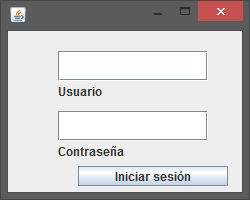
\includegraphics[width=.4\textwidth]{images/gui/Login}
		\caption{Pantalla de Control de Acceso}
\end{figure}
%%%%%%%%%%%%%%%%%%%%%%%%%%%%%%
\section{Doctor}
En la pantalla principal del doctor tenemos cuatro funciones en total: Generar receta, Consultar expediente m\'edico, Generar expediente m\'edico y Modificar expediente m\'edico. Si se desea regresar al login, debe darle click al bot\'on "`Cerrar sesi\'on"'.


%%%%%%%%%%%%%%%%%%%%%%%%%%%%%%
\subsection{Consultar expediente m\'edico}
Aqu\'i lo \'unico que tiene qu\'e hacer es introducir el CURP del paciente del cual se quiera conocer su expediente m\'edico. Posteriormente debe dar click en el bot\'on "`Buscar"', y si hay un expediente encontrado con el CURP encontrado, se desplegar\'a en todos los dem\'as campos de la pantalla, la informaci\'on correspondiente, de lo contrario se mostr\'a un mensaje diciendo que no se encontr\'o ning\'un expediente con el CURP ingresado.

Finalmente para regresar al men\'u principal, debe dar click en el bot\'on "`Regresar"'.

En la figura 6.2 podemos apreciar la pantalla correspondiente a \'esta funci\'on.

\begin{figure}[htbp!]
		\centering		
	\end{figure}
\begin{figure}[htbp!]
\centering
		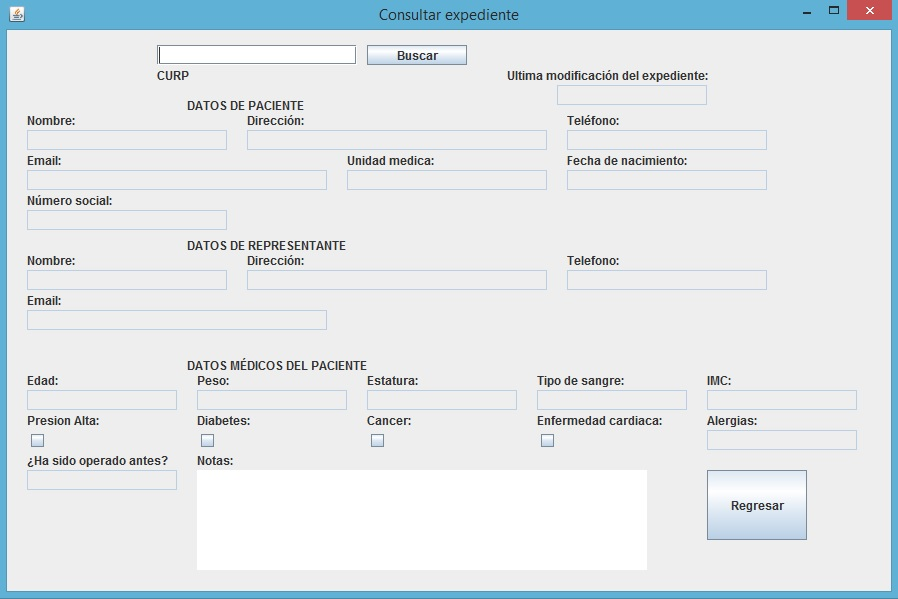
\includegraphics[width=.8\textwidth]{images/gui/IUConsultaExp}
		\caption{Consultar expediente}
\end{figure}
%%%%%%%%%%%%%%%%%%%%%%%%%%%%%%
\subsection{Modificar expediente m\'edico}
Aqu\'i lo \'unico que tiene qu\'e hacer es introducir el CURP del paciente del cual se quiera modificar su expediente m\'edico. Posteriormente debe dar click en el bot\'on "`Buscar"', y si hay un expediente encontrado con el CURP encontrado, se desplegar\'a en todos los dem\'as campos de la pantalla, la informaci\'on correspondiente, de lo contrario se mostr\'a un mensaje diciendo que no se encontr\'o ning\'un expediente con el CURP ingresado.

\'Esta funcionalidad es bastante similar a la de consultar expediente, s\'olo que aqu\' algunos campos de informaci\'on ya se pueden modificar. Al darle click al bot\'on "`Modificar"', el sistema sobreescribir\'a la informaci\'on anterior del expediente con la que est\'a actualmente en el formulario de la pantalla, as\'i que si se accede a \'esta funci\'on pero no se modific\'o ning\'un campo, en realidad no habr\'a ning\'un cambio en el expediente

Finalmente para regresar al men\'u principal, debe dar click en el bot\'on "`Regresar"'.

En la figura 6.3 podemos apreciar la pantalla correspondiente a \'esta funci\'on.

\begin{figure}[htbp!]
		\centering		
	\end{figure}
\begin{figure}[htbp!]
\centering
		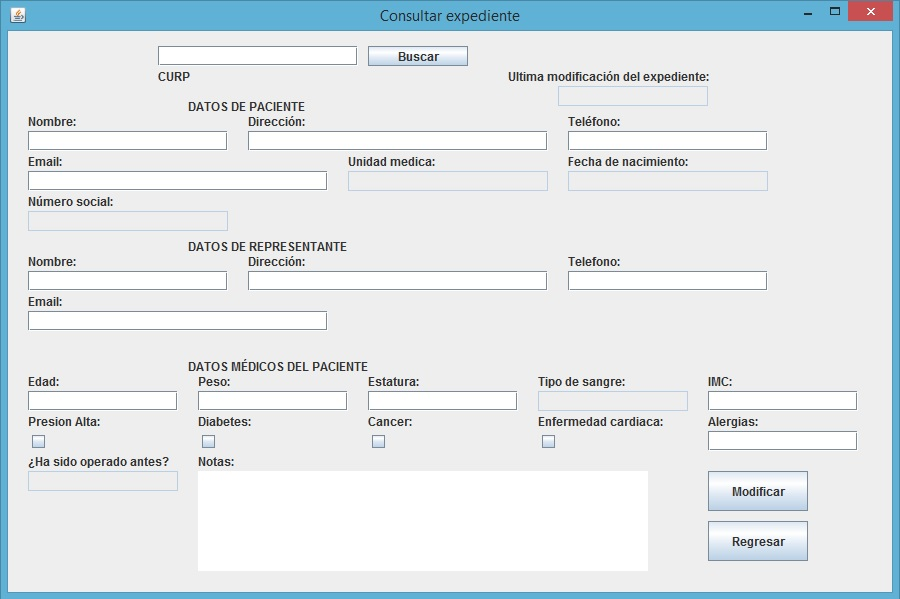
\includegraphics[width=.8\textwidth]{images/gui/IUModificaExp}
		\caption{Modificar expediente}
\end{figure}


%%%%%%%%%%%%%%%%%%%%%%%%%%%%%%
\subsection{Generar expediente m\'edico}

Aqu\'i se encuentran varios campos vac\'ios que constituyen la informaci\'on que debe contener el nuevo expediente. Debe llenar todos los campos, especialmente el del CURP, ya que con \'este dato es con el que ser\'a posible consultar y modificar el expediente en futuras ocasiones.
Cuando se haya ingresado toda la informaci\'on requerida, se debe dar click al bot\'on  "`Generar"', para registrar el expediente en el sistema

Finalmente para regresar al men\'u principal, debe dar click en el bot\'on "`Regresar"'.

En la figura 6.4 podemos apreciar la pantalla correspondiente a \'esta funci\'on.

\begin{figure}[htbp!]
		\centering		
	\end{figure}
\begin{figure}[htbp!]
\centering
		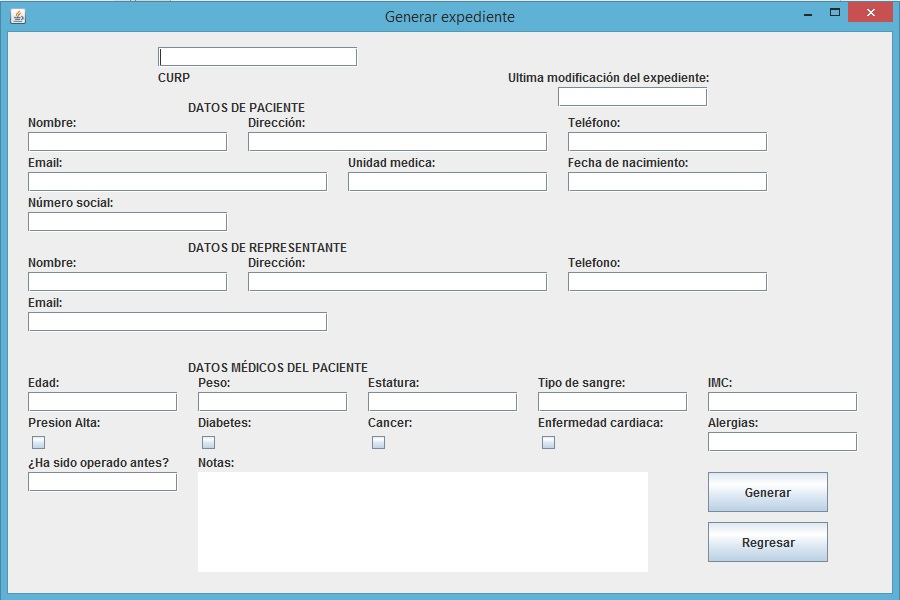
\includegraphics[width=.9\textwidth]{images/gui/IUGeneraExp}
		\caption{Generar expediente}
\end{figure}

%%%%%%%%%%%%%%%%%%%%%%%%%%%%%%
\subsection{Generar receta}
Aqu\'i podr\'a seleccionar los medicamentos que quiere que est\'en en su receta. Para poner uno debe escribir el ID de ese medicamento con el cual est\'a registrado en el sistema y la dosis o alguna nota que desea agregar. Si desconoce el ID de alg\'un medicamento puede hacer una b\'usqueda ya sea por nombre o por sustancia activa con la herramienta que se encuentra en la parte superior de la pantalla.

Si desea agregar m\'as de un medicamento, debe dar click en la opci\'on "`Agregar medicamento"' para agregar una fila m\'as de datos. Por otro lado si quiere quitar un medicamento que ya ingres\'o, puede darle click en la opci\'on "`Eliminar"' de la fila donde est\'e el medicamento que desea eliminar.

Finalmente para regresar al men\'u principal, debe dar click en el bot\'on "`Regresar"'.

En la figura 6.5 podemos apreciar la pantalla correspondiente a \'esta funci\'on.

\begin{figure}[htbp!]
		\centering		
	\end{figure}
\begin{figure}[htbp!]
\centering
		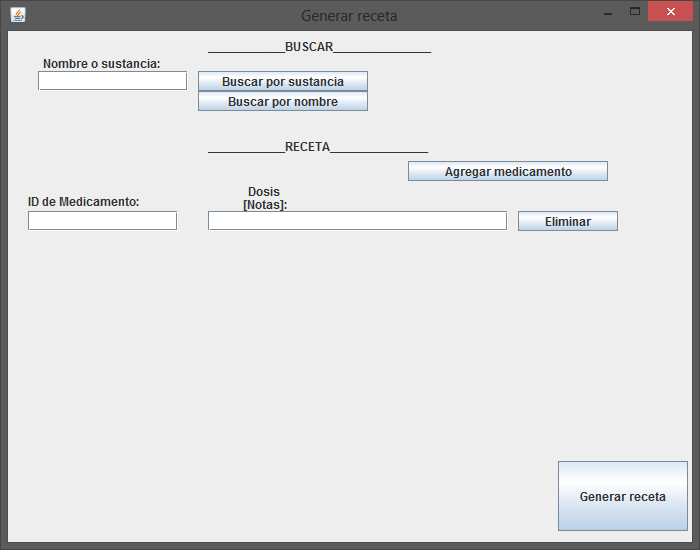
\includegraphics[width=.9\textwidth]{images/gui/IUCrearReceta}
		\caption{Creaci\'on de receta}
\end{figure}


%%%%%%%%%%%%%%%%%%%%%%%%%%%%%%
\section{Proveedor}
En el m\'odulo del proveedor hay una \'unica funci\'on, que es aumentar el stock de un medicamento ya registrado. Simplemente es necesario ingresar el ID del medicamento al cual se le quiere aumentar el stock, y la cantidad de unidades que se suministran de tal medicamento. Posteriormente al dar click en "`Agregar"' se actualizar\'a el stock del medicamento ingresado, en el sistema y aparecer\'a un mensaje mostrando la cantidad de unidades que hay en el sistema tras la actualizaci\'on realizada.


Finalmente para regresar a la pantalla de control de acceso, debe dar click en el bot\'on "`Cerrar sesi\'on"'.

En la figura 6.6 se puede apreciar la interfaz de \'este m\'odulo.


\begin{figure}[htbp!]
		\centering		
	\end{figure}
	
\begin{figure}[htbp!]
\centering
		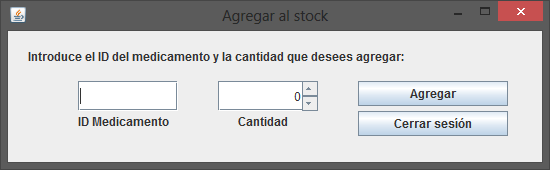
\includegraphics[width=.7\textwidth]{images/gui/IUProv}
		\caption{Pantalla de proveedor}
\end{figure}

%%%%%%%%%%%%%%%%%%%%%%%%%%%%%%
\section{Cajero}
En \'este m\'odulo, al igual que el proveedor, el cajero tiene una s\'ola funci\'on y es registrar como "`Pagada"' una transacci\'on en el sistema que est\'e pendiente. Para ello es necesario el ID de la transacci\'on, misma que ya debe estar registrada en el sistema. Posteriormente se debe ingresar la cantidad que el cajero recibo por parte del cliente. Tras \'esto, debe dar click en el bot\'on "`Pagar"' y el sistema verificar\'a si hay dinero suficiente en la caja para dar cambio, de lo contrario mostrar\'a una advertencia. Si s\'i hay dinero suficiente, registrar\'a la transacci\'on como "`Pagada"' en el sistema.


Finalmente para regresar a la pantalla de control de acceso, debe dar click en el bot\'on "`Cerrar sesi\'on"'.

En la figura 6.7 se puede apreciar la interfaz de \'este m\'odulo.

\begin{figure}[htbp!]
		\centering		
	\end{figure}
\begin{figure}[htbp!]
\centering
		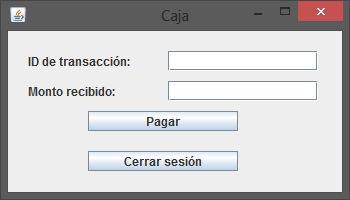
\includegraphics[width=.5\textwidth]{images/gui/IUCaja}
		\caption{Pantalla de cajero}
\end{figure}


%%%%%%%%%%%%%%%%%%%%%%%%%%%%%%
\section{Dependiente}
El m\'odulo del dependiente tiene tres funciones: 
\begin{itemize}
\item Registrar compra de medicamentos.
\item Consultar el stock de un medicamento
\item Buscar un medicamento
\end{itemize}

%%%%%%%%%%%%%%%%%%%%%%%%%%%%%%
\subsection{Compra}
En \'este m\'odulo se podr\'a registrar una compra de medicamentos y generar un recibo de pago.
Primero es necesario ingresar el ID del medicamento que se quiere agregar y la cantidad. \'Este \'ultimo dato debe ser un n\'umero. Si se desea agregar m\'as de un medicamento, al darle click al bot\'on "`Agregar"' se agregar\'a una nueva fila donde se podr\'an ingresar los datos de otro medicamento. Si es necesario se puede eliminar una fila completa haciendo click en el bot\'on "`Eliminar"' de la fila que se desea quitar. Posteriormente al dar click en el bo\'ton "`Comprar"', el sistema procesar\'a la informaci\'on ingresada.
Si hay alg\'un medicamento que no est\'a registrado en el sistema, se mostrar\'a un mensaje diciendo que uno o m\'as medicamentos no est\'an registrados. Si todos los medicamentos est\'an registrados se mostrar\'a una ventana con un resumen de lo que se desea comprar. Al dar click en la opci\'on "`Aceptar"' se registrar\'a la transacci\'on pendiente en el sistema y se imprimir\'a un recibo de pago. Tras \'esto el sistema volver\'a a la pantalla de compra.

En la figura 6.8 se puede apreciar la pantalla de \'esta funci\'on.
\begin{figure}[htbp!]
		\centering		
	\end{figure}
\begin{figure}[htbp!]
\centering
		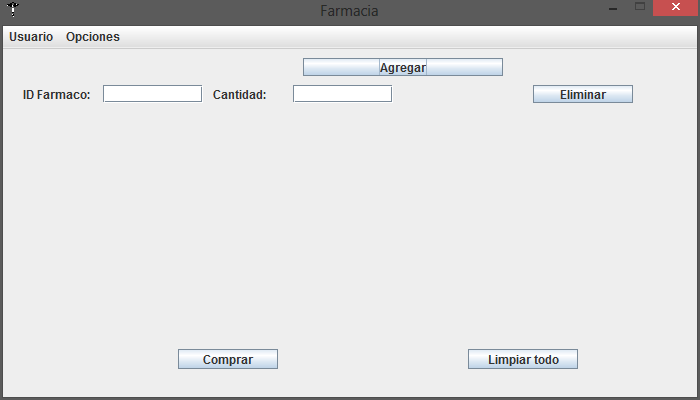
\includegraphics[width=.7\textwidth]{images/gui/IUCompra}
		\caption{Pantalla de compra}
\end{figure}


%%%%%%%%%%%%%%%%%%%%%%%%%%%%%%
\subsection{Consultar stock}
\'Esta funci\'on es bastante sencilla. S\'olo debe ingresarse el ID del medicamento del cual se quiera conocer el stock, entonces se mostrar\'a la cantidad en unidades que se encuentra en el stock del medicamento ingresado. Si el sistema no encuentra ning\'un medicamento registrado con el ID ingresado, mostrar\'a una advertencia diciendo que verifique sus datos.

En la figura 6.9 se puede apreciar la pantalla de \'esta funci\'on.

\begin{figure}[htbp!]
		\centering		
	\end{figure}
\begin{figure}[htbp!]
\centering
		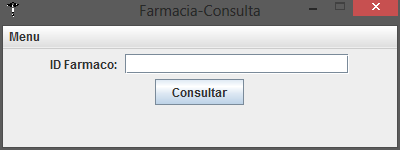
\includegraphics[width=.5\textwidth]{images/gui/IUConsulta}
		\caption{Pantalla de consulta}
\end{figure}


%%%%%%%%%%%%%%%%%%%%%%%%%%%%%%
\subsection{Buscar medicamento}
Aqu\'i se podr\'a buscar un medicamento de dos formas: Por nombre y por sustancia activa. S\'olo basta con ingresar la informaci\'on en el campo que corresponda y dar click en el bot\'on asociado con el campo ingresado. Despu\'es de \'esto, se mostrar\'a una ventana con una tabla (ver Figura 6.10) que muestra la informaci\'on de los medicamentos encontrados con ese nombre o sustancia activa, incluyendo la cantidad que se encuentra en stock de cada medicamento hallado.

En la figura 6.11 se puede apreciar la pantalla de \'esta funci\'on.

\begin{figure}[htbp!]
		\centering		
	\end{figure}
\begin{figure}[htbp!]
\centering
		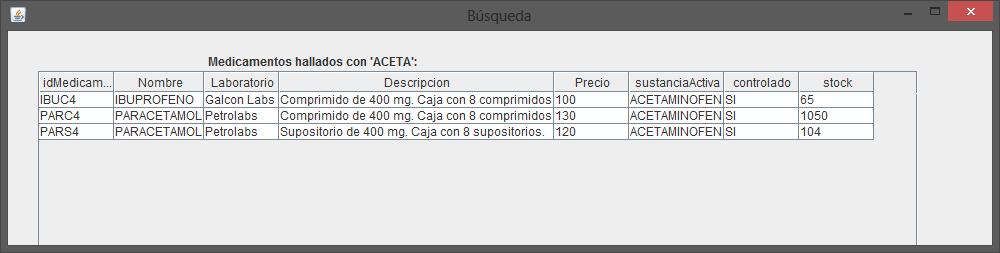
\includegraphics[width=.9\textwidth]{images/gui/IUResultados}
		\caption{Tabla de resultados}
\end{figure}
\begin{figure}[htbp!]
		\centering		
	\end{figure}
\begin{figure}[htbp!]
\centering
		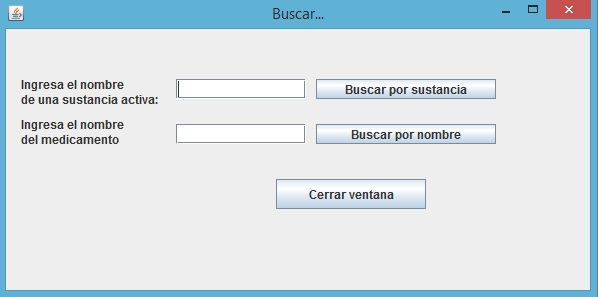
\includegraphics[width=.7\textwidth]{images/gui/IUBusqueda}
		\caption{Pantalla de b\'usqueda}
\end{figure}



%%%%%%%%%%%%%%%%%%%%%%%%%%%%%%
\section{Administrador}
En \'este m\'odulo se tienen dos funciones para el administrador: Registrar un usuario y registrar un medicamento.

%%%%%%%%%%%%%%%%%%%%%%%%
\subsection{Registrar un usuario}
Aqu\'i se deben ingresar tres datos esenciales: Nombre de usuario, contraseña y rol de la cuenta. La contraseña se tiene qu\'e escribir dos veces y el rol se selecciona desde una lista desplegable. Posteriormente debe dar click en la opci\'on "`Registrar"'. Ambas contraseñas deben ser id\'enticas y el usuario ingresado no debe estar registrado, para poder registrar exitosamente la cuenta de usuario.


Para regresar a la pantalla anterior, debe dar click en el bot\'on "`Regresar"'.

En la figura 6.12 se puede observar la figura asociada a \'esta funci\'on.

\begin{figure}[htbp!]
		\centering		
	\end{figure}
\begin{figure}[htbp!]
\centering
		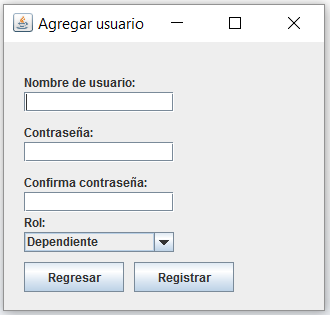
\includegraphics[width=.5\textwidth]{images/gui/IUAgregarUsuario}
		\caption{Pantalla de registro de usuario}
\end{figure}
%%%%%%%%%%%%%%%%%%%%%%%%
\subsection{Registrar un medicamento}
En \'esta funci\'on se deben agregar siete datos relacionados con un medicamento, que son: id, nombre, laboratorio, descripci\'on, sustancia activa, precio y una bandera que indica si es controlado o no.
Una vez habiendo ingresado \'esta informaci\'on, debe dar click en la opci\'on "`Registrar"', y tras un mensaje de \'exito, el medicamento quedar\'a registrado en el sistema. En caso de que ya haya un medicamento registrado con el ID ingresado se mostrar\'a una advertencia que lo indique.


Para regresar a la pantalla anterior, debe dar click en el bot\'on "`Regresar"'.

En la figura 6.13 se puede observar la figura asociada a \'esta funci\'on.

\begin{figure}[htbp!]
		\centering		
	\end{figure}
\begin{figure}[htbp!]
\centering
		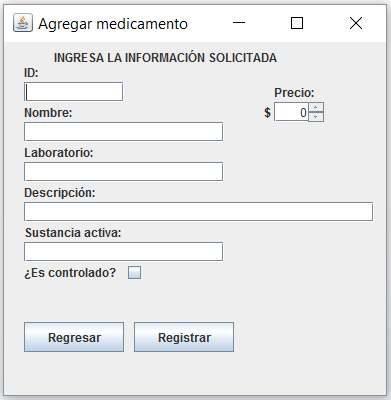
\includegraphics[width=.5\textwidth]{images/gui/IUAgregarMedicamento}
		\caption{Pantalla de registro de medicamento}
\end{figure}

